\documentclass[10pt,conference]{IEEEtran}

\ifCLASSINFOpdf
	\usepackage[pdftex]{graphicx}
	%\graphicspath{{./figs/}}
	\DeclareGraphicsExtensions{.pdf,.jpeg,.png}
\else
	\usepackage[dvips]{graphicx}
	%\graphicspath{{./figs/}}
	\DeclareGraphicsExtensions{.eps}
\fi

\usepackage[cmex10]{amsmath}
\usepackage[tight,footnotesize]{subfigure}
\usepackage{xcolor}
\usepackage[lined,ruled]{algorithm2e}

\usepackage[latin1]{inputenc}
\usepackage{float}
\usepackage{tikz}
\usetikzlibrary{shapes}
\usetikzlibrary{arrows}

\usepackage[]{algorithm2e}
\usepackage{amsmath}
\raggedbottom

\newtheorem{property}{Property}
\newtheorem{proposition}{Proposition}
\newtheorem{theorem}{Theorem}
\newtheorem{conjecture}{Conjecture}
\newtheorem{question}{Question}
\newtheorem{definition}{Definition}
\newtheorem{corollary}{Corollary}

\makeatletter
\pgfdeclareshape{datastore}{
\inheritsavedanchors[from=rectangle]
\inheritanchorborder[from=rectangle]
\inheritanchor[from=rectangle]{center}
\inheritanchor[from=rectangle]{base}
\inheritanchor[from=rectangle]{north}
\inheritanchor[from=rectangle]{north east}
\inheritanchor[from=rectangle]{east}
\inheritanchor[from=rectangle]{south east}
\inheritanchor[from=rectangle]{south}
\inheritanchor[from=rectangle]{south west}
\inheritanchor[from=rectangle]{west}
\inheritanchor[from=rectangle]{north west}
\backgroundpath{
    %  store lower right in xa/ya and upper right in xb/yb
\southwest \pgf@xa=\pgf@x \pgf@ya=\pgf@y
\northeast \pgf@xb=\pgf@x \pgf@yb=\pgf@y
\pgfpathmoveto{\pgfpoint{\pgf@xa}{\pgf@ya}}
\pgfpathlineto{\pgfpoint{\pgf@xb}{\pgf@ya}}
\pgfpathmoveto{\pgfpoint{\pgf@xa}{\pgf@yb}}
\pgfpathlineto{\pgfpoint{\pgf@xb}{\pgf@yb}}
 }
}
\makeatother

\newcommand{\riham}[1]{{\color{red}{#1}}}
\newcommand{\james}[1]{{\color{blue}{#1}}}


\begin{document}

\title{Anti-Money Laundering Visualization}
\author{
\IEEEauthorblockN{Debopriyo Ghosh}
\IEEEauthorblockA{Rutgers University\\}
 \email{dg1114@scarletmail.rutgers.edu}
\and
\IEEEauthorblockN{Nish Patel}
\IEEEauthorblockA{Rutgers University\\}
 \email{nsp124@scarletmail.rutgers.edu}
\and
\IEEEauthorblockN{Jahnavi Manchala}
\IEEEauthorblockA{Rutgers University\\}
 \email{jm2658@scarletmail.rutgers.edu}
}
\maketitle
\begin{abstract}
\textnormal{With massive graph networks, the analyst can not visualize or analyze the graph using a traditional visualization. Despite this, analysts will need to perform an ad-hoc review of accounts to identify potential accounts of interest. Visualizing the data with a graph city solves this problem by allowing analysts to see the entire graph and perform analysis one building at a time. We used the graph city architecture introduced by James Abello, H. Zhang, Daniel Nakhimovich, Chengguizi Han, and Mridul Aanjaneya.\cite{Abello2022GigaGC}}
\end{abstract}
\providecommand{\keywords}[1]
{
  \small	
  \textbf{\textit{Keywords---}} #1
}
\keywords{Money Laundering Detection, Graph Cities, Data Visualization, Synthetic Laundering Transactions, Neo4j, Neovis, PySpark, Monitoring Transactions
}
%\onecolumn \maketitle \normalsize \vfill

\IEEEpeerreviewmaketitle
%%%%%%%%%%%%%%%%%%%%%%%%%%%%%%%%%%%%%%%%%%%%%%%%%%%%%%%%%%%%%%%%%%%%%%%%%%%%%%%%%%%%%%%%%%%%%%%%%%%%%%%%%
\section{Introduction}\label{sec:1. Introduction}
%%%%%%%%%%%%%%%%%%%%%%%%%%%%%%%%%%%%%%%%%%%%%%%%%%%%%%%%%%%%%%%%%%%%%%%%%%%%%%%%%%%%%%%%%%%%%%%%%%%%%%%%%
\textnormal{
\setlength{\parindent}{2em}Money laundering detection is a critical issue in the financial sector, where the stakes are exceptionally high due to the potential for large-scale financial crimes. Real financial transaction data, which is pivotal in identifying and combating such illicit activities, is highly confidential and difficult to obtain for privacy reasons. This confidentiality is necessary to protect the personal and financial information of individuals and institutions but simultaneously poses a significant challenge for regulatory bodies and financial institutions striving to detect and prevent money laundering. As a result, developing effective detection systems often relies on sophisticated techniques that can work with limited or synthesized data, while still accurately identifying suspicious activities without violating privacy norms and regulations. IBM has developed a simulation model to generate synthetic transactions. The simulation includes simulated money laundering and these transactions are labeled in the dataset.
}

\textnormal{
 Our project aims to provide analysts with a visualization tool to perform an ad-hoc analysis of financial transaction data to identify possible accounts of interest. Once the accounts of interest are found, we aim to help the analyst review financial transactions conducted by the accounts and their related accounts.
}


\section{Dataset Description }\label{sec:1 Dataset Description. }
%%%%%%%
\textnormal{The dataset has been generated by IBM and is based on a virtual world inhabited by individuals, companies, and banks. Individuals interact with other individuals and companies. Likewise, companies interact with other companies and with individuals. These interactions can take many forms, e.g. purchase of consumer goods and services, purchase orders for industrial supplies, payment of salaries, repayment of loans, and more. These financial transactions are generally conducted via banks, i.e. the payer and receiver both have accounts, with accounts taking multiple forms from checking to credit cards to bitcoin.
The data generator that created the data not only models illicit activity, but also tracks funds derived from illicit activity through arbitrarily many transactions. We use a higher illicit ratio (more laundering) for our project.\cite{IBMML}
The dataset (17 GB in size) contains 180 million records (100 bytes per record), 2.1 million distinct bank accounts, 15 distinct currencies
, and 7 distinct payment formats. The data was generated via the IBM simulation from August 1, 2022 to November 5, 2022.}\cite{Dataset}

\begin{figure}[htp]
    \centering
    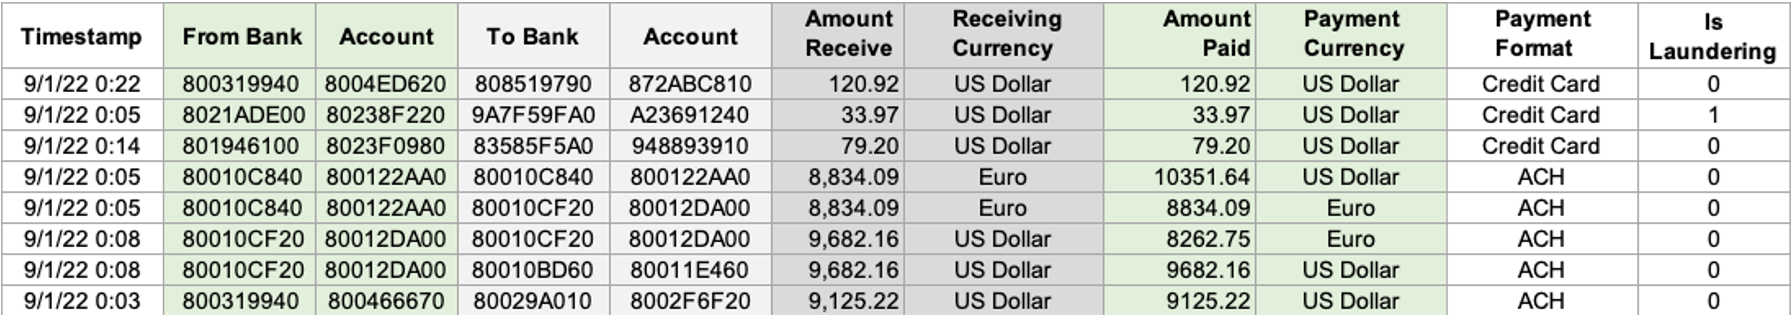
\includegraphics[width=8cm]{imgs/snapshot.png}
    \caption{Dataset Record Structure}
    \label{fig:DataFlowDiagram}
\end{figure}

\begin{figure}[htbp]
    \centering
    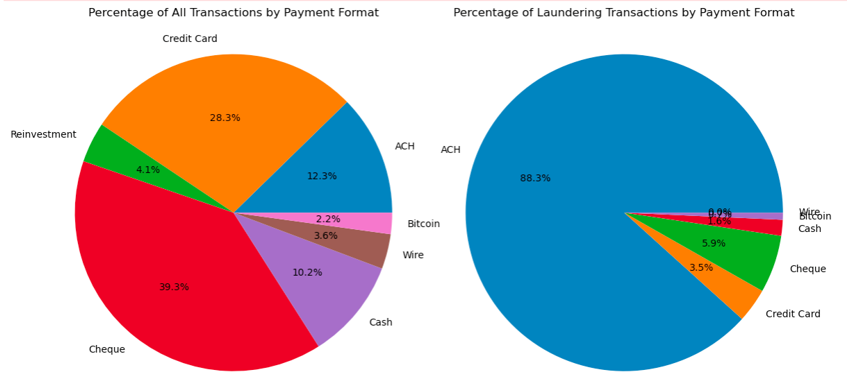
\includegraphics[width=7cm]{imgs/payment.png}
    \caption{Transactions in Payment Format}
    \label{fig:Data23}
\end{figure}

\begin{figure}[h]
    \centering
    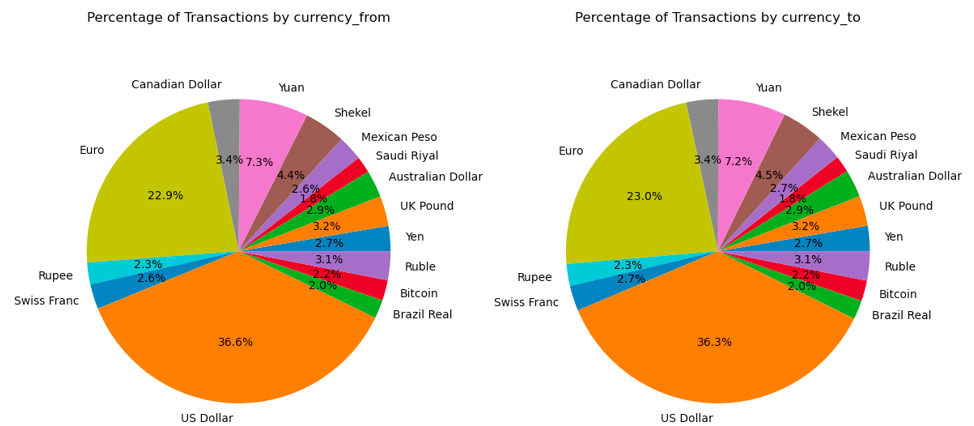
\includegraphics[width=8cm]{imgs/currency.png}
    \caption{Transactions in Currency Format}
    \label{fig:Diagram}
\end{figure}

\vspace{\baselineskip}

\section{Questions to Answer}\label{sec: Questions to Answer.}
%%%%%%%%%%%%%%%%%%%%%%%%%%%%%%%%%%%%%%%%%%%%%%%%%%%%%%%%%%%%%%%%%%%%%%%%%%%%%%%%%%%%%%%%%%%%%%%%%%%%%%%%%%
\textnormal{Currently, the industry relies heavily on manual analysis of transactions in order to flag and review fraudulent transactions with a high false positive rate. As data volume has increased and new digital currencies have been introduced, the challenge of identifying potential money-laundering transactions with legacy rules-based has increased exponentially. The three fundamental questions we are asking are:}

\begin{enumerate}
\item{
What is the best data type for financial transaction data?}
\item{
How can we help analysts perform ad-hoc analysis of financial transaction data to identify possible accounts of interest?}
\item{
Once the accounts of interest are found, how can we help the analyst review financial transactions conducted by the accounts and their related accounts?}

\end{enumerate}
\vspace{\baselineskip} 

\section{Methodology}\label{sec: Methodology}
%%%%%%%%%%%%%%%%%%%%%%%%%%%%%%%%%%%%%%%%%%%%%%%%%%%%%%%%%%%%%%%%%%%%%%%%%%%%%%%%%%%%%%%%%%%%%%%%%%%%%%%%%%
\vspace{\baselineskip} 
\begin{itemize} 
\item To answer question 1, a literature review was conducted to identify the current trends in the space. Legacy rules-based analysis relied on the table data structure within relational databases and pre-defined thresholds for identifying potential fraudulent
transactions. Transactions over ten thousand dollars must be reported to the IRS. The key component that was missing from these systems was the ability to easily view the context of the transactions and the accounts that money is being transferred from or to.
As graph analytics\cite{GraphAnalytics} have evolved due to the rise of social networks, the financial industry has also embraced graphs to model financial transactions as a series of relationships to provide the missing context. Based on the literature review, we decided to utilize the graph data structure to model our data. Given the need to store, query, and visualize graph data, the data was converted
\cite{Neo4j}into nodes and edges via a Python script and imported into a graph database (Neo4j) that can natively handle the relationships and provide an efficient query mechanism.


\begin{figure}[H]
\begin{center}
    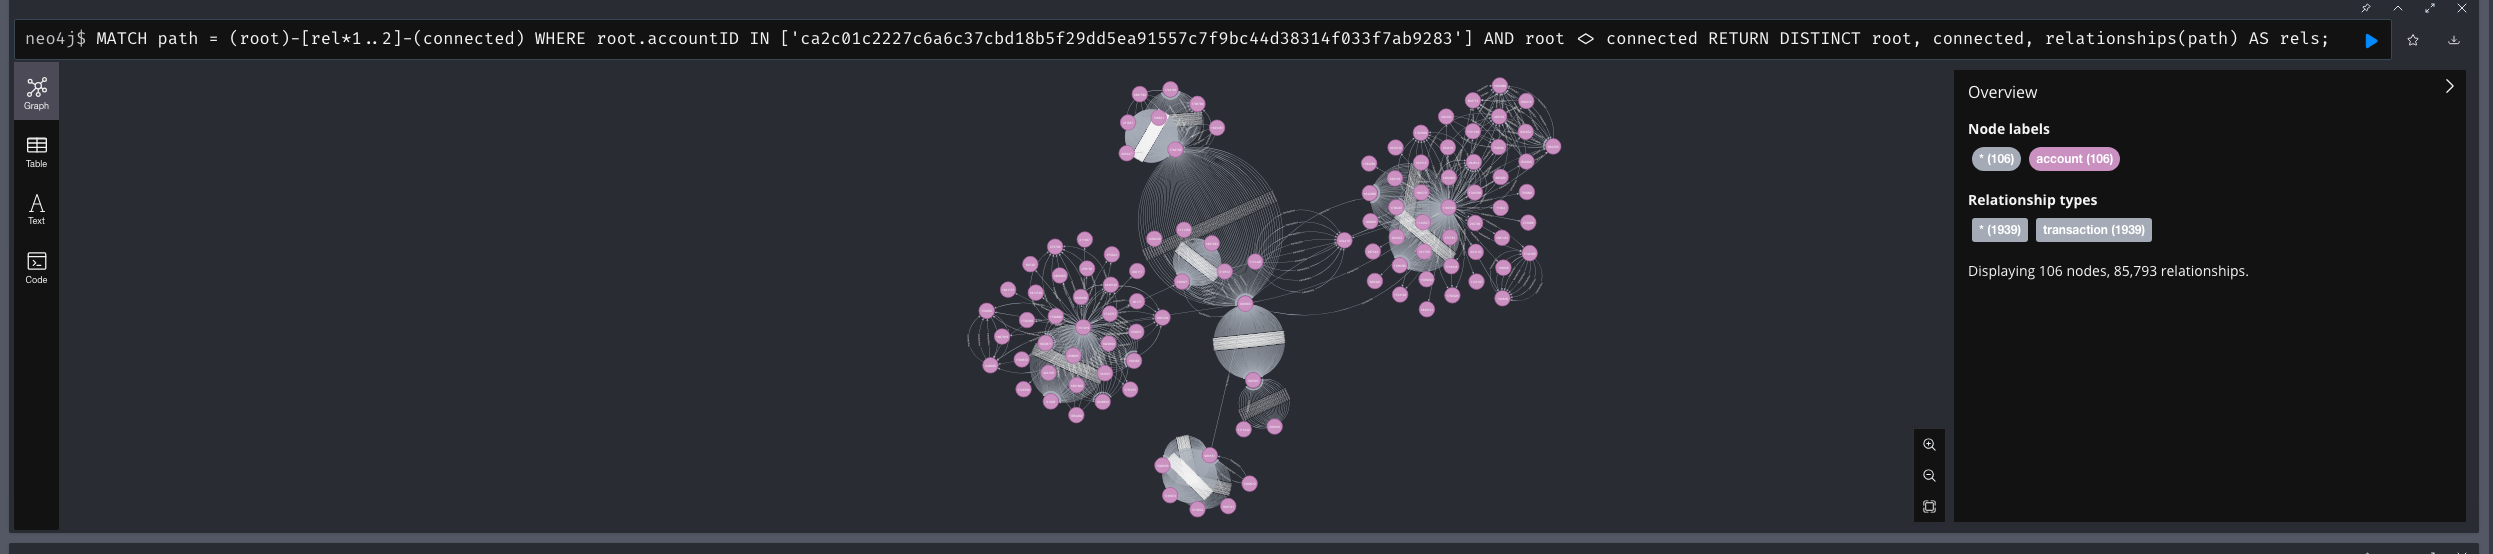
\includegraphics[width=8cm]{imgs/neo4j.png}
    \caption{Neo4j Database}
    \centering
\end{center}
\end{figure}

\item To answer question 2, the main issue to address was the screen bottleneck. With massive graph networks, the analyst can not visualize or analyze the graph using a traditional visualization. Despite this, analysts will need to perform an ad-hoc review of accounts to identify potential accounts of interest. Visualizing the data with a graph city solves this problem by allowing analysts to
see the entire graph and perform analysis one building at a time. We used the graph city architecture introduced by James Abello, H. Zhang, Daniel Nakhimovich, Chengguizi Han, and Mridul Aanjaneya.\cite{Abello2022GigaGC}\cite{Abello2021GraphCT}\cite{Abello2020GraphW}\cite{Abello2013FixedPO}

\begin{figure}[htp]
    \centering
    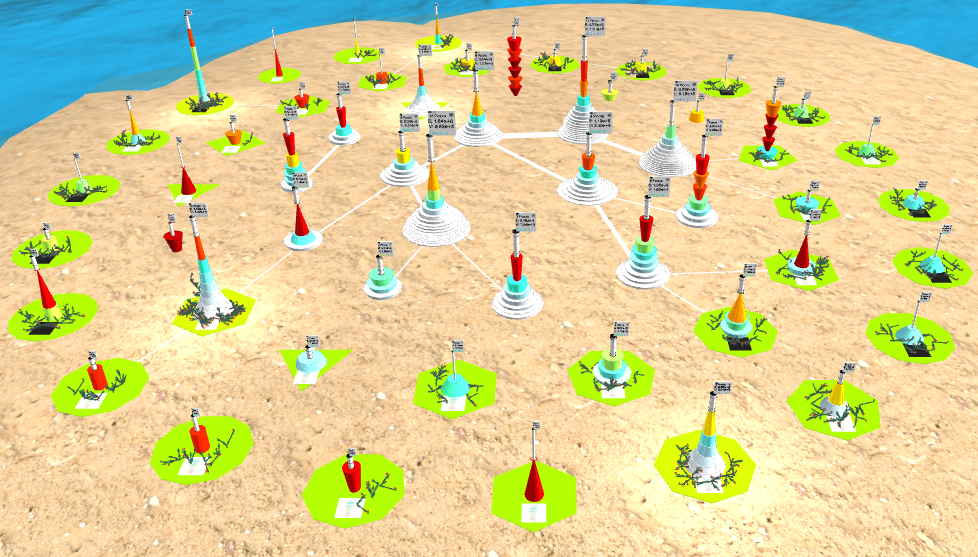
\includegraphics[width=7cm]{imgs/graph_city.png}
    \caption{Graph City Buildings}
    \label{fig:DataFlowDiagram}
\end{figure}


\begin{figure}[H]
\begin{center}
    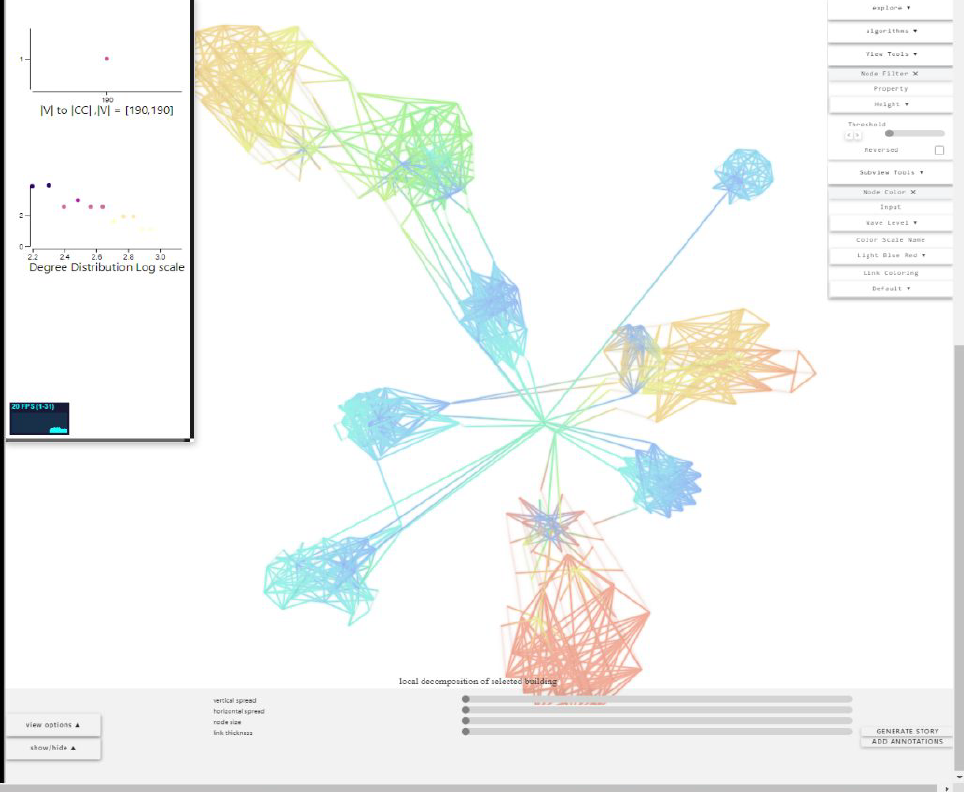
\includegraphics[width=7cm]{imgs/graph_node.png}
    \caption{Graph Nodes}
    \centering
\end{center}
\end{figure}

\item To answer question 3, we needed to figure out how to leverage Neo4j's advanced capabilities to allow analysts to view transactions for particular accounts and their related accounts. This was done by creating a search application that allows the user to filter on
certain key attributes and visualize a graph of an account (or series of accounts).

\begin{figure}[H]
\begin{center}
    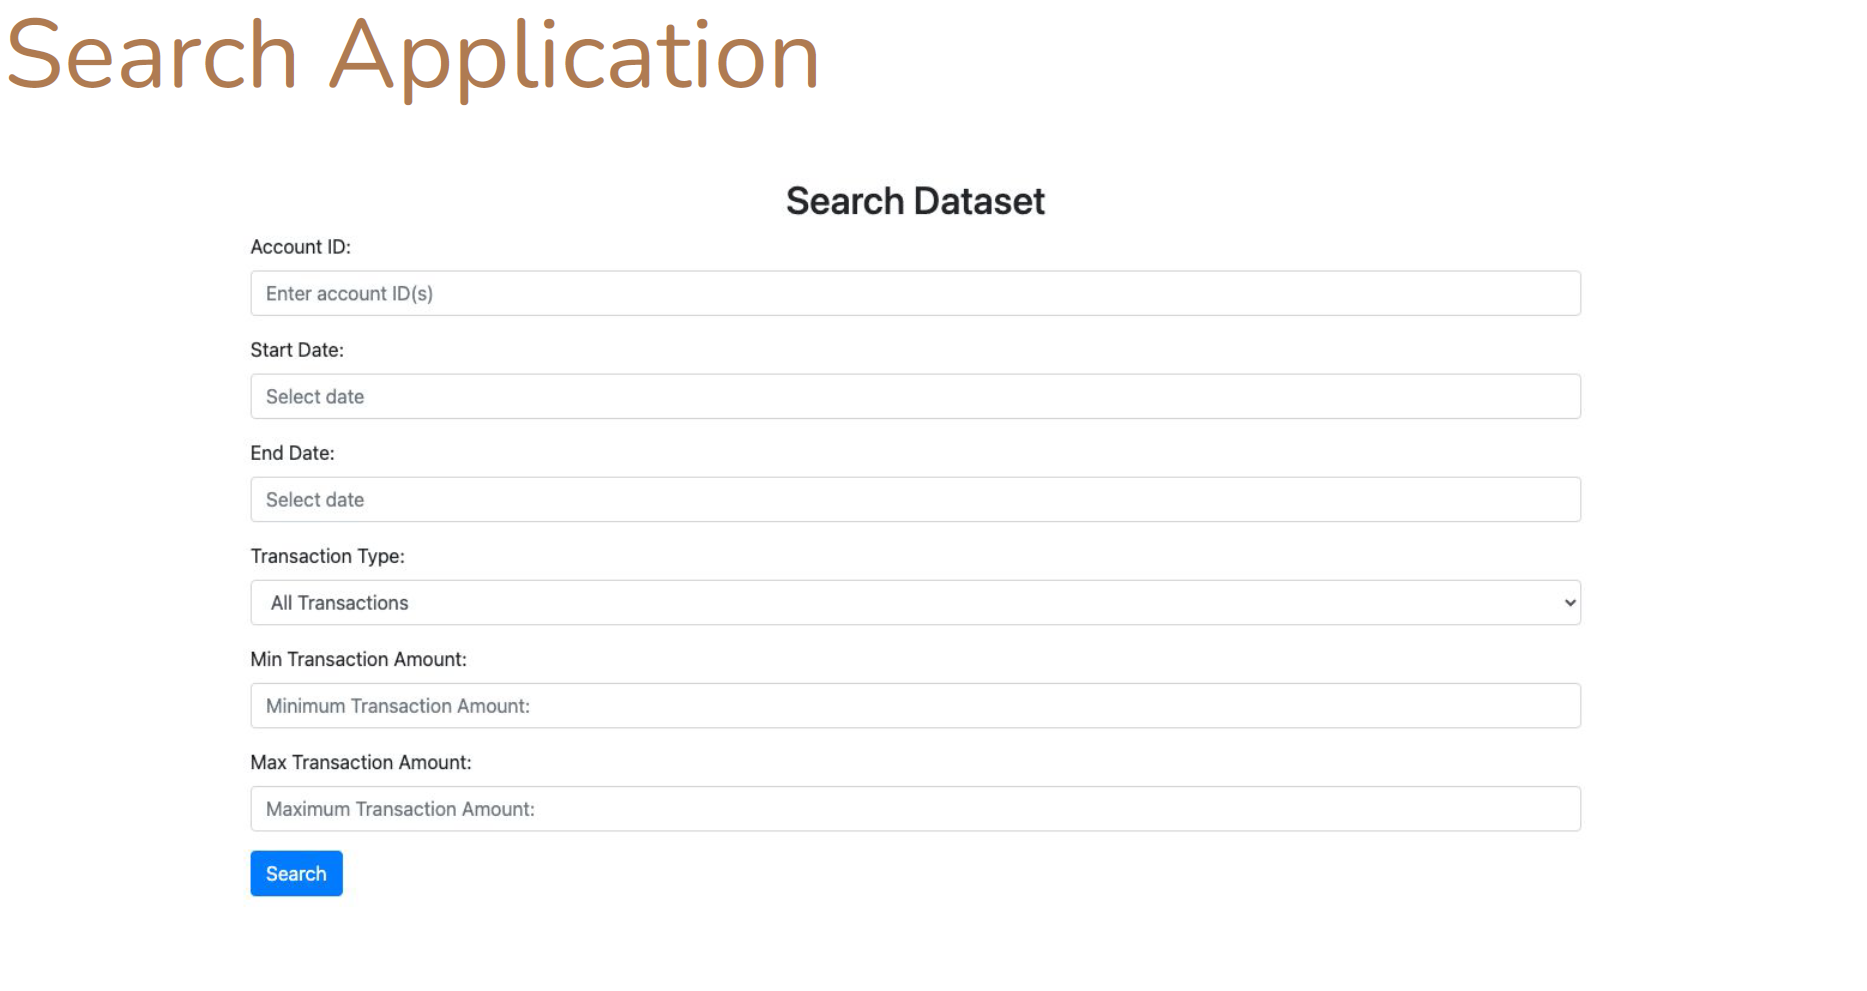
\includegraphics[width=8cm]{imgs/searchapp.png}
    \caption{Search Application}
    \centering
\end{center}
\end{figure}

Once the query is submitted, a graph visualization is rendered that shows all transactions by that account and also any transaction by accounts that the account sent money to (depth 2).\cite{Neovis}

\begin{figure}[H]
\begin{center}
    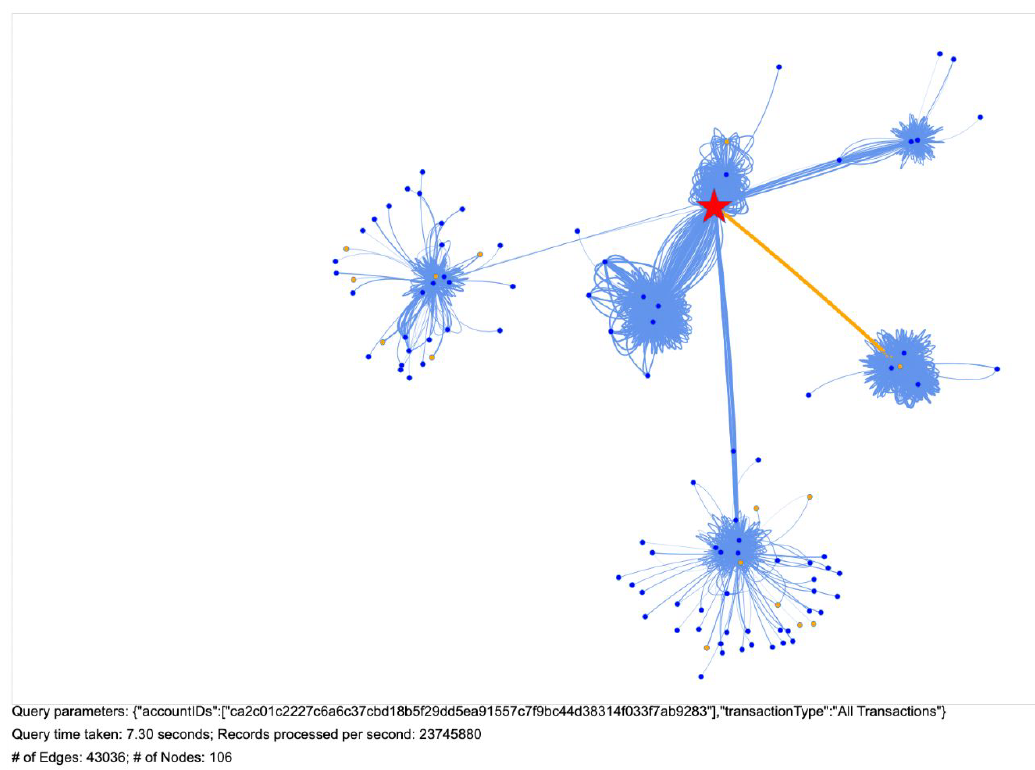
\includegraphics[width=8cm]{imgs/queryresult.png}
    \caption{Query Result}
    \centering
\end{center}
\end{figure}

An interesting finding is that communities of interest are readily apparent when visualizing the accounts through the search application.


\end{itemize}


\vspace{\baselineskip} 

\section{Implementation }\label{sec: Implementation}
%%%%%%%%%%%%%%%%%%%%%%%%%%%%%%%%%%%%%%%%%%%%%%%%%%%%%%%%%%%%%%%%%%%%%%%%%%%%%%%%%%%%%%%%%%%%%%%%%%%%%%%%%%
\textnormal{ 
\begin{itemize}
\item We performed data cleaning and preprocessing steps to prepare a CSV to be used in the analysis.
\begin{itemize}
\item Check for nulls (no null values in any column)
\item Calculate conversion rates from each currency to USD and prepare a new column of payments in US Dollars
\item Create a unique id by hashing bank + '\_' + account
\item Convert timestamp columns into integer year, month, day, hour, minute columns to save space
\item Output a 'clean' CSV for use in visualizations and modeling
\end{itemize}
\item We use the clean data to create two CSVs with the account data (accounts.csv) and the transaction data (transactions.csv)
\item We import these account and transaction information data into Neo4j and build a database.
\item We build a web application that primarily uses client-server architecture with MVT (Model, View, Template) design pattern. 
\begin{figure}[htp]
    \centering
    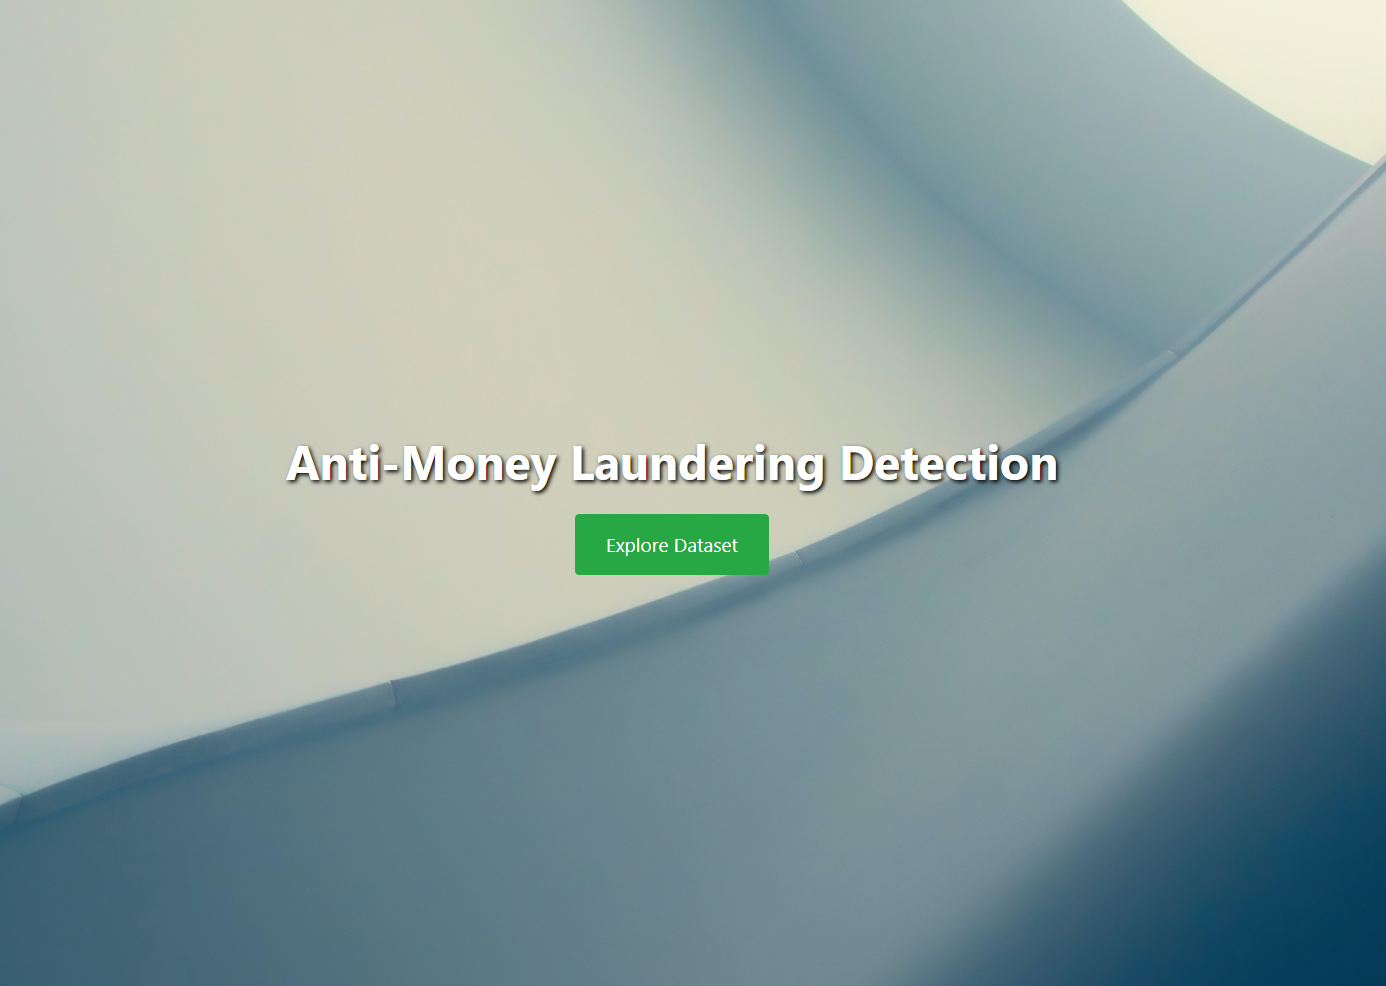
\includegraphics[width=6cm]{imgs/home.png}
    \caption{Web App home page}
    \label{fig:DataFlowDiagram}
\end{figure}
\item We format the dataset as aml.txt and aml\_label.csv for importing into the Graph City backend.
\item We use the Graph City Architecture to generate the Graph City for our dataset.
\begin{figure}[htbp]
    \centering
    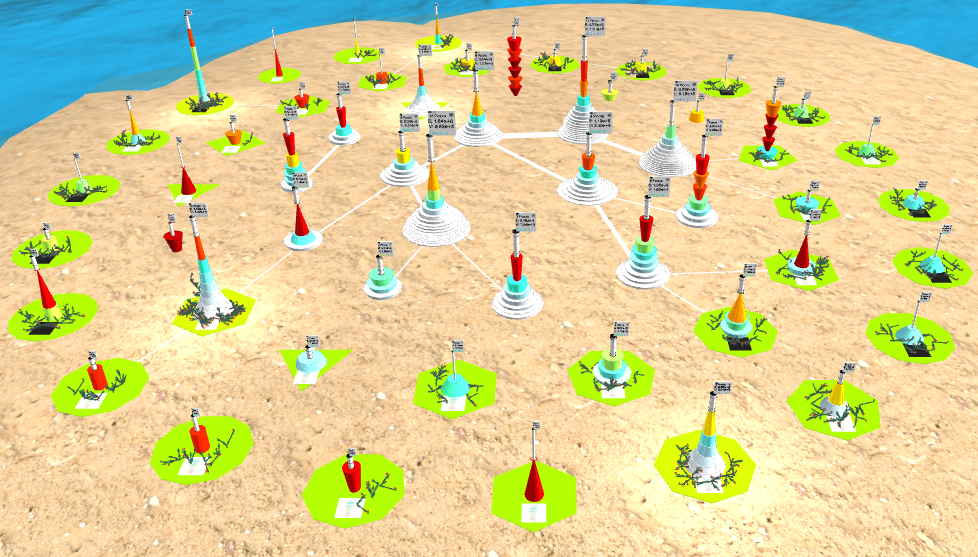
\includegraphics[width=7cm]{imgs/graph_city2.png}
    \caption{Generated Graph City for AML}
    \label{fig:DataFlowDiagram}
\end{figure}
\item We link the Graph City Front-End to our application.
\end{itemize}
}
\textnormal{
The application is used to connect to Graph City and provide a high-level visual representation of the data. The user can now explore the network clusters that can be used to initiate an analysis of the data:}
\begin{itemize}
    \item Explore a cluster in Graph City
    
    \begin{figure}[htp]
    \centering
    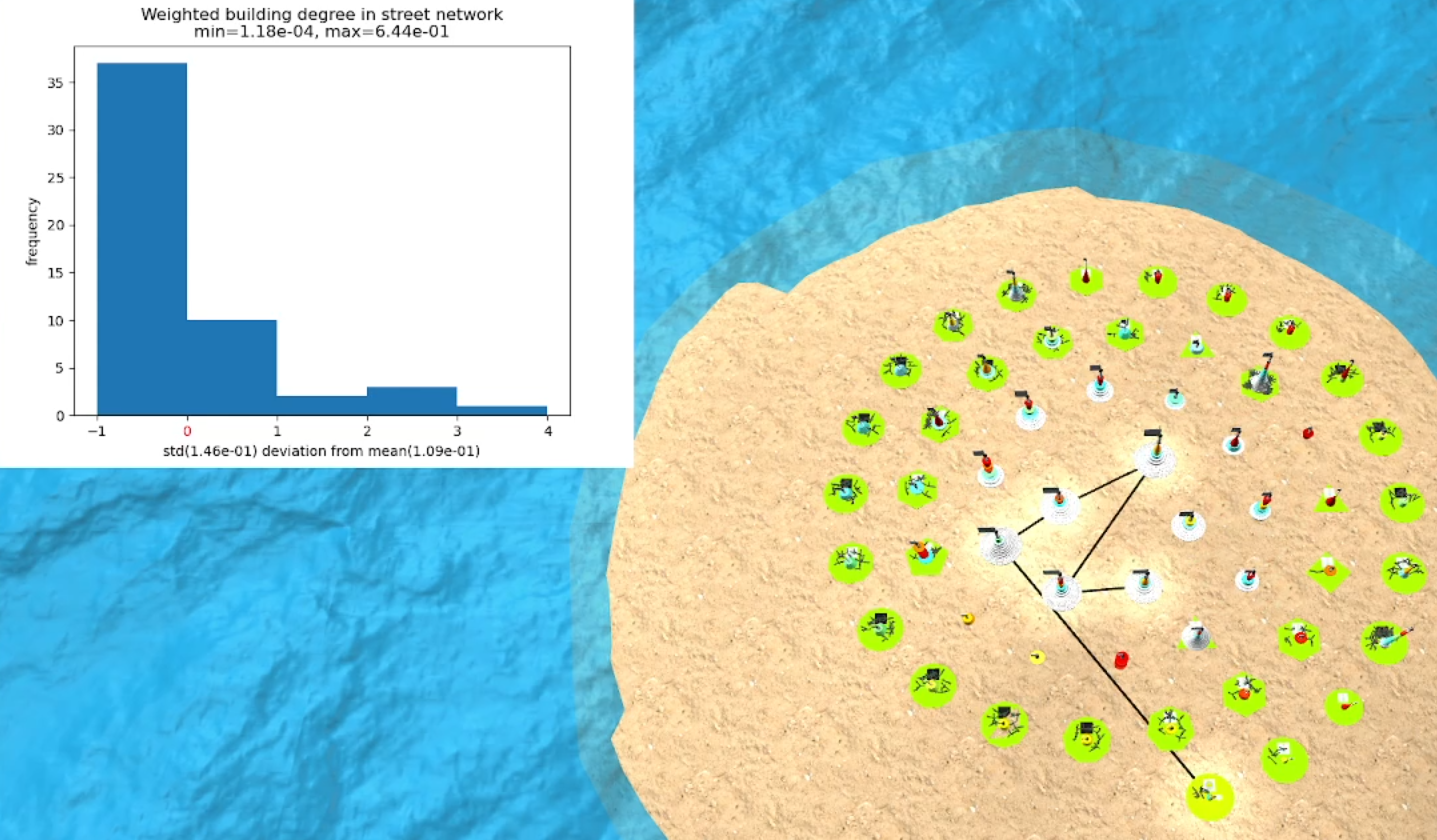
\includegraphics[width=7cm]{imgs/exploration.png}
    \caption{Data Exploration}
    \label{fig:FlowDiagram}
    \end{figure}
    
    \begin{figure}[htp]
    \centering
    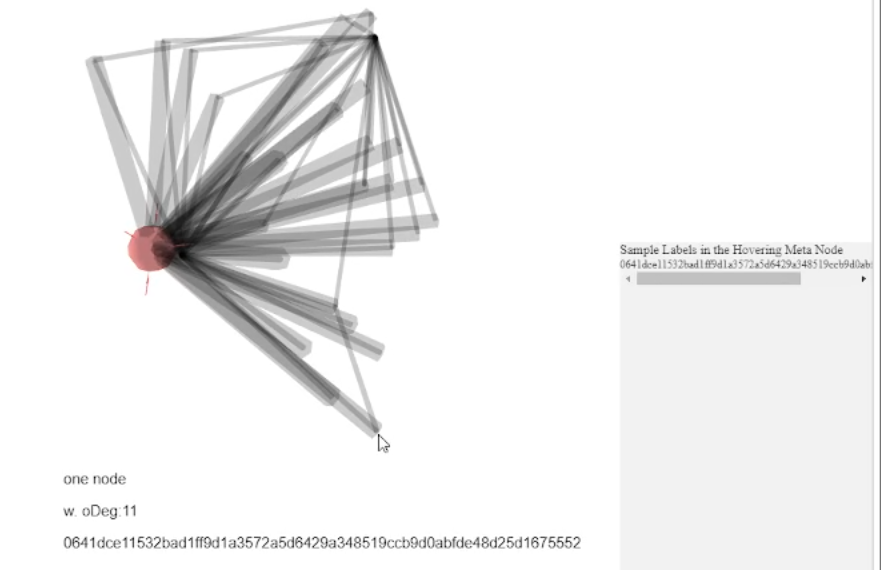
\includegraphics[width=7cm]{imgs/nodeexlore.png}
    \caption{Node Exploration}
    \label{fig:DataFDiagram}
    \end{figure}
    \item Click on a node to redirect to our app to query Neo4j
    \item Generate the cluster visualization of connected nodes
    
    \begin{figure}[htp]
    \centering
    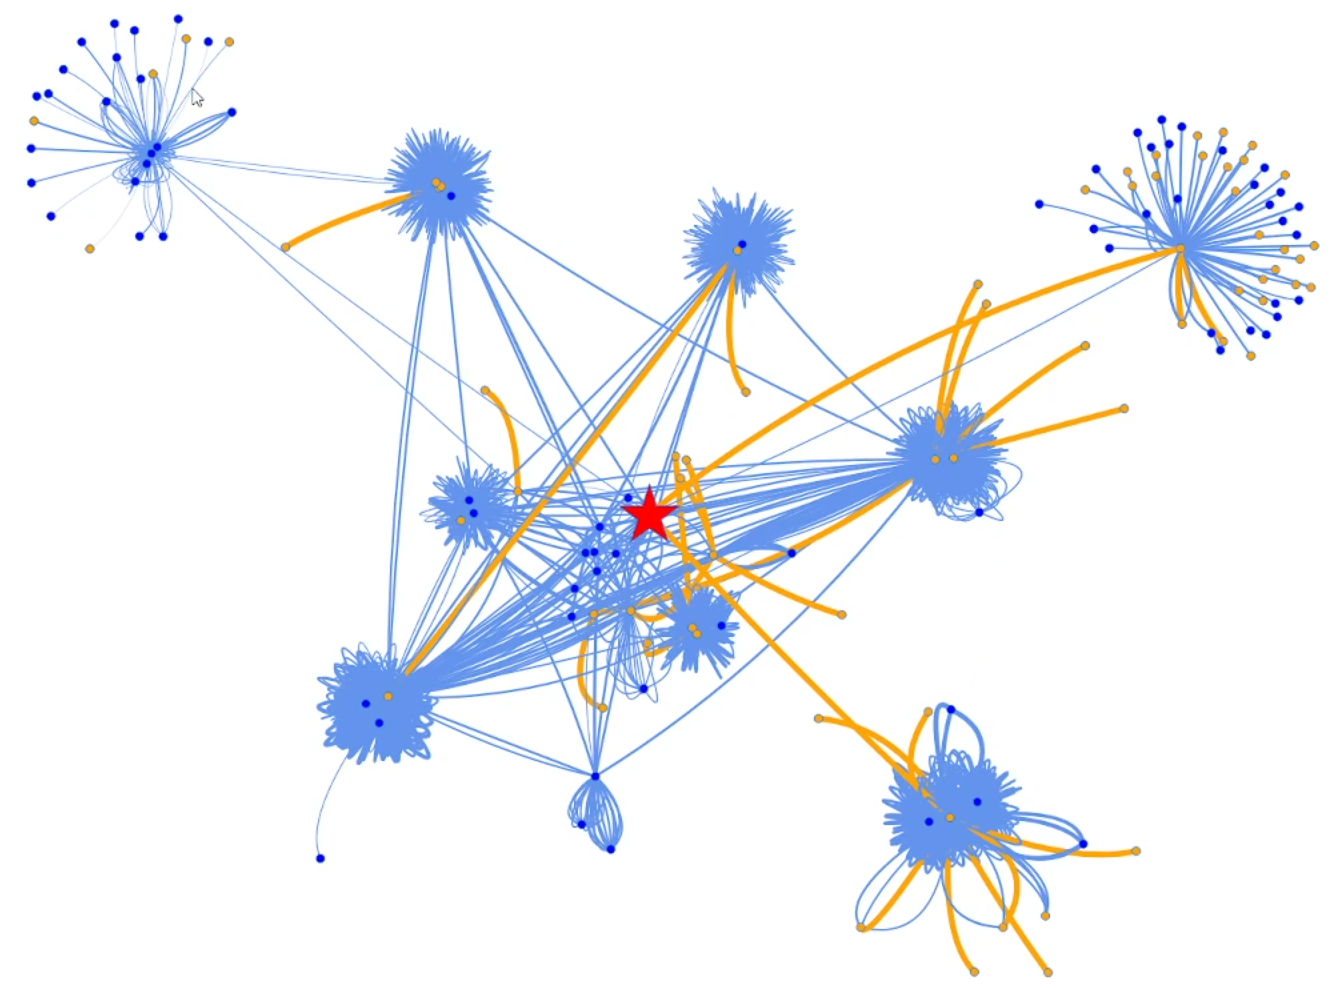
\includegraphics[width=7cm]{imgs/laundering.png}
    \caption{Connected Node Exploration}
    \label{fig:Data}
    \end{figure}
    \item Find laundering transactions and follow laundering chains
    
\end{itemize}

\section{Architecture }\label{sec: Architecture.}
%%%%%%%%%%%%%%%%%%%%%%%%%%%%%%%%%%%%%%%%%%%%%%%%%%%%%%%%%%%%%%%%%%%%%%%%%%%%%%%%%%%%%%%%%%%%%%%%%%%%%%%%%%
\vspace{\baselineskip} 
\textnormal{
The user interface was developed with HTML5, CSS, Javascript, and Node.js. The database was created using Neo4j and Neovis was used to visualize the data. Graph City interface was implemented using the GitHub repository\cite{GraphCities}  Additional libraries and dependencies include:
}
\begin{itemize}
  \item Python
  \item PySpark
  \item Jupyter Notebook
  \item Pandas
  \item Matplotlib
  \item Numpy
\end{itemize}

\begin{figure}[htbp]
    \centering
    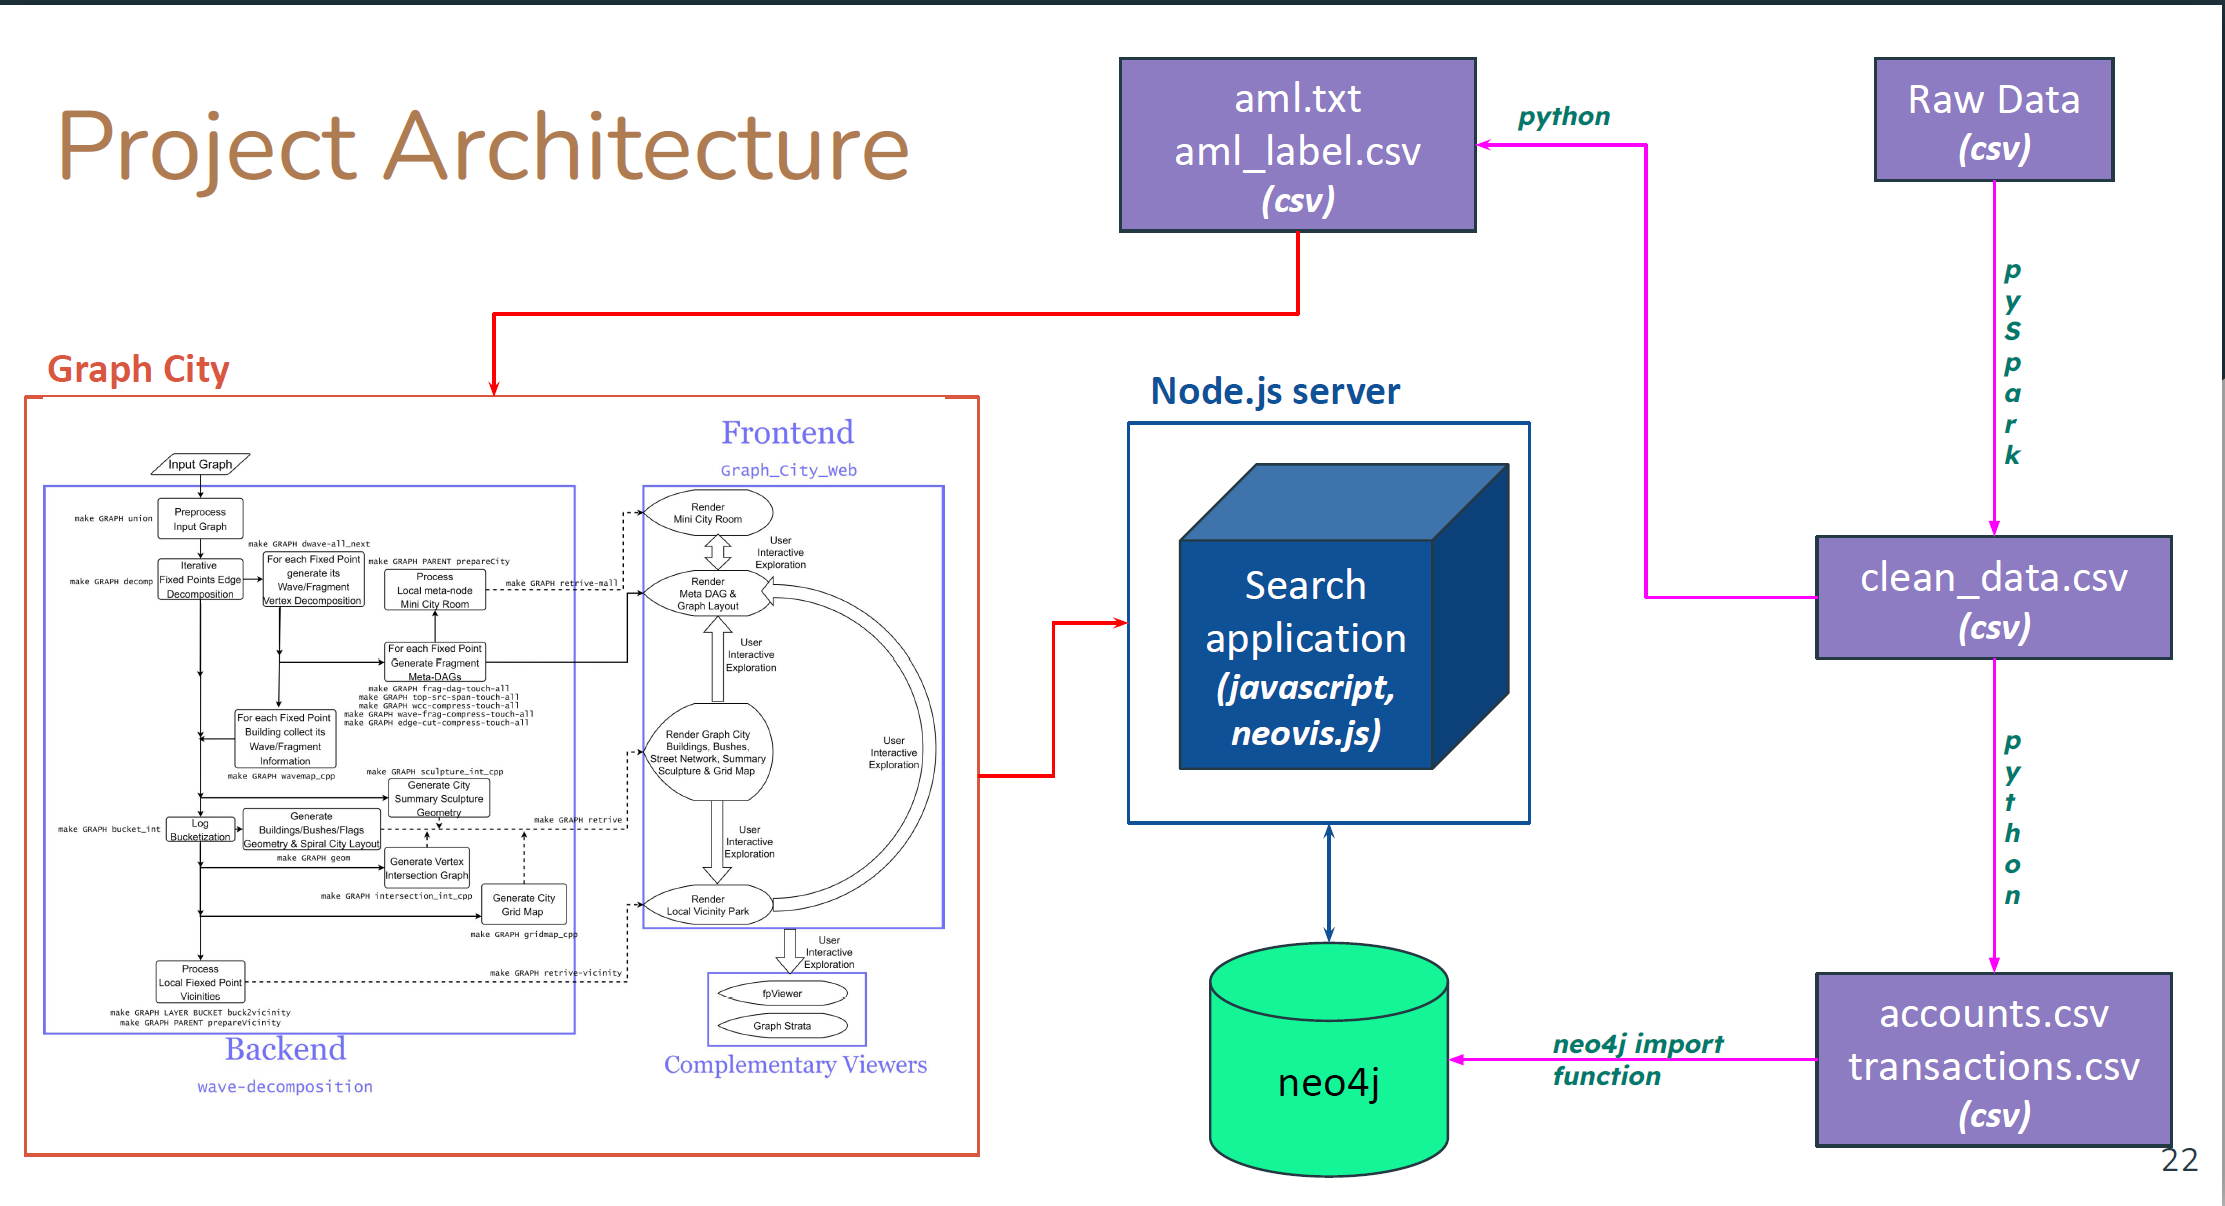
\includegraphics[width=8cm]{imgs/architecture.png}
    \caption{Project Architecture}
    \label{fig:Dataad}
\end{figure}



\section{Project Timeline}\label{sec:5. Project Timeline}
%%%%%%%%%%%%%%%%%%%%%%%%%%%%%%%%%%%%%%%%%%%%%%%%%%%%%%%%%%%%%%%%%%%%%%%%%%%%%%%%%%%%%%%%%%%%%%%%%%%%%%%%%%
\textnormal{}

\begin{figure}[htbp]
    \centering
    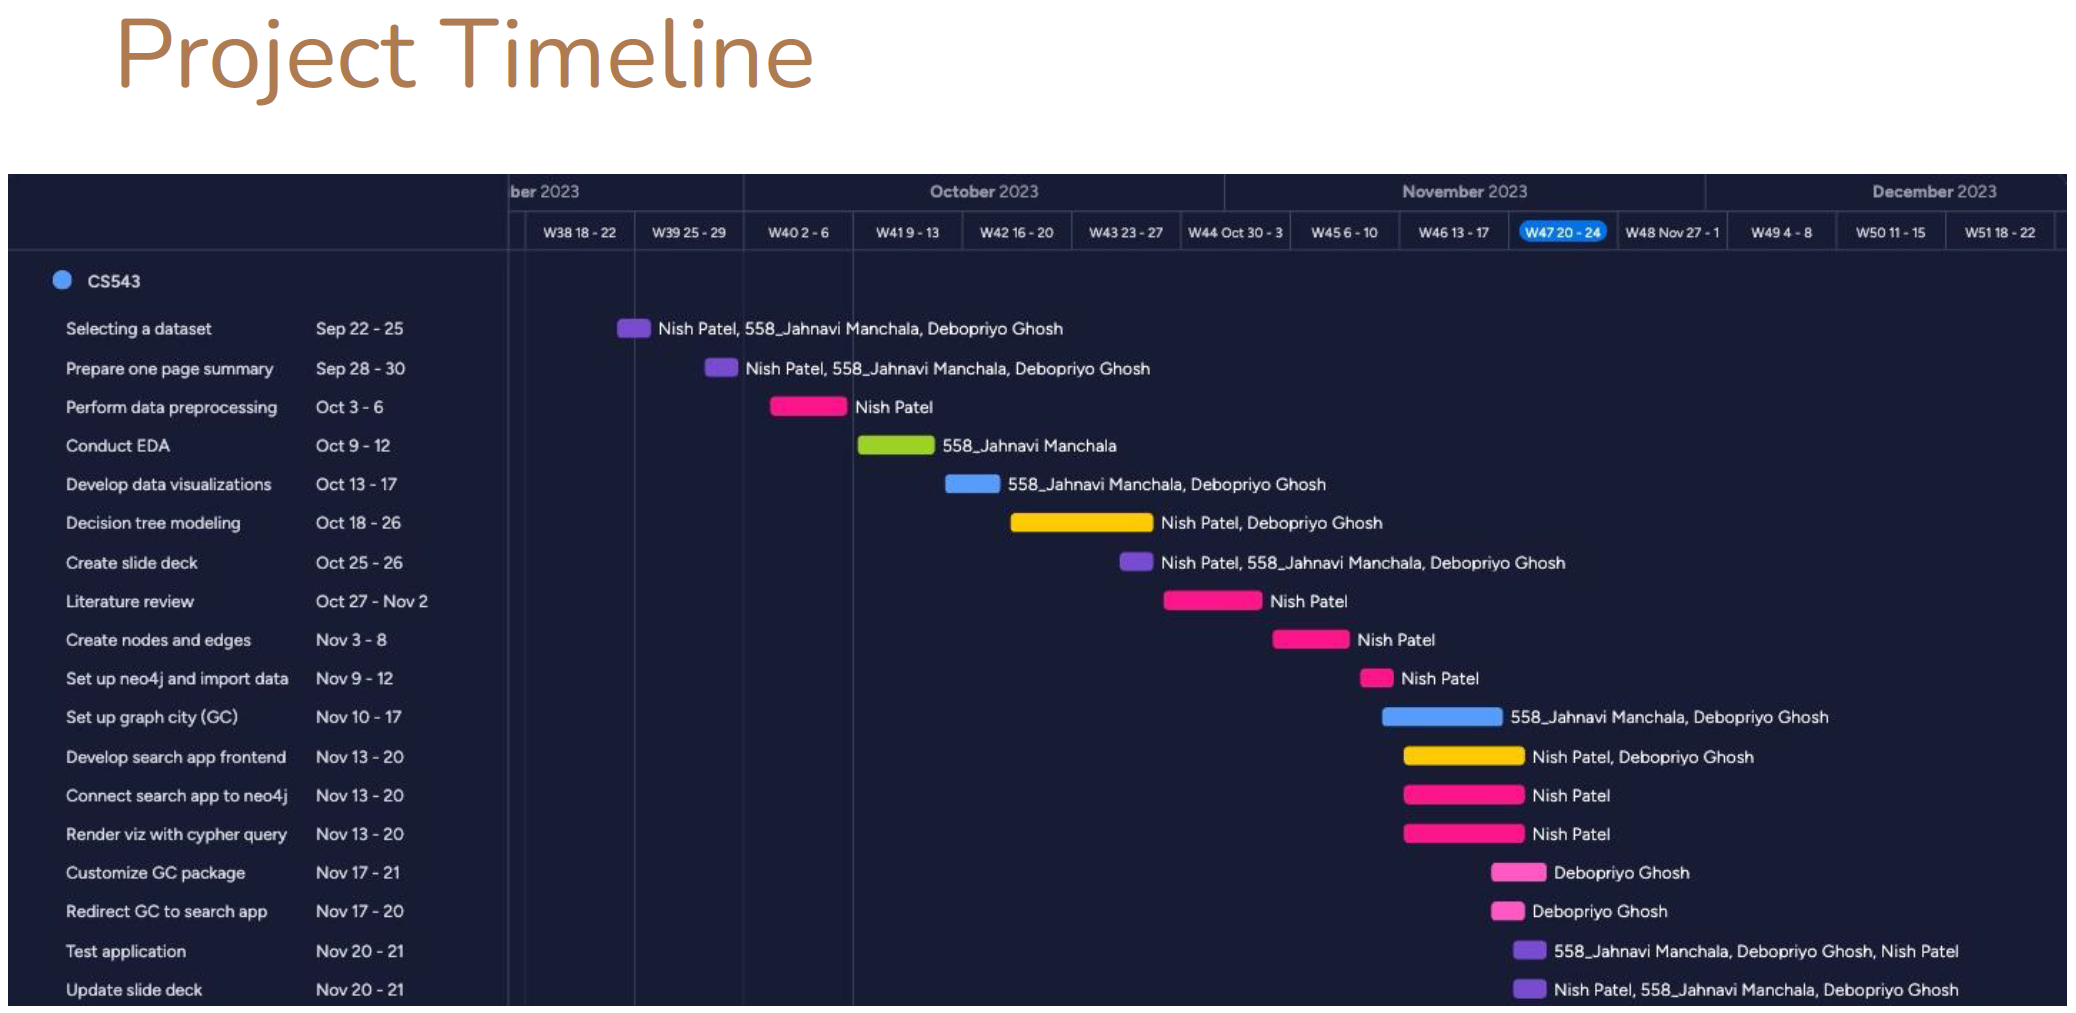
\includegraphics[width=8cm]{imgs/timeline.png}
    \caption{Project Timeline and Gantt Chart}
    \label{fig:timeline}
\end{figure}


Division of Work:
\begin{itemize}
\item{
Nish Patel: Data Processing, Background Processing, UI, Visualizations, Testing }
\item{
Debopriyo Ghosh: UI, Graph-City Implementation, Integration, Testing, Reporting }
\item{
Jahnavi Manchala: Data Visualizations, Graph-City Exploration, Testing}

\end{itemize}

\section{Future work.}\label{sec: Future work}
%%%%%%%%%%%%%%%%%%%%%%%%%%%%%%%%%%%%%%%%%%%%%%%%%%%%%%%%%%%%%%%%%%%%%%%%%%%%%%%%%%%%%%%%%%%%%%%%%%%%%%%%%%

\begin{itemize}
    \item{Attempt to utilize a graph convolutional neural network to predict if a transaction is a money laundering transaction or not.}
    \item{A key benefit of using graphs as the data type (as mentioned in the question \(1\)) is to be able to utilize the relationships between accounts to identify potential fraud}
    \item{Given 90\%+ false positive rates using traditional methods, graph convolutional neural networks should be able to utilize the context of the relationships to produce lower false positive rates.}
\end{itemize}

\bibliographystyle{IEEEtran}
\bibliography{paper.bib}

\end{document}


